\chapter{Di cosa stiamo parlando}

In questo primo capitolo ci occuperemo di una semplice introduzione generale al Deep Learning, concentrandoci sul suo apetto a livello sociale ed effettuando anche dei riferimenti storici. Ovviamente tutto ciò che verrà trattato in questo capitolo, viene trattato con un livello di dettaglio, notevolmente ridotto, sorvolando anche su alcune cose, ma ciò può essere un ottimo punto di partenza, per poter approfondire diversi aspetti, sviluppando la curiosità del lettore. I modelli di Deep Learning sono oggi onnipresenti: li troviamo negli ospedali per la diagnosi automatica, in agricoltura per il monitoraggio delle colture, nella domotica per la gestione intelligente degli ambienti, negli assistenti virtuali, nei sistemi di rilevamento delle frodi, nella manutenzione predittiva degli impianti industriali e in molto altro.

\section{Applicazioni}

Le applicazioni del Deep Learning sono estremamente varie e in continua espansione, pertanto sarebbe pressocché impossibile elencarli tutti, di seguito elenchiamo solo alcuni dei possibili esempi di campi di applicazione:

\begin{itemize}
    \item Traduzioni automatiche (es. Google Translate, Google Lens, DeepL, Wordvice AI, ecc\dots);
    \item Sistemi di guida autonoma (es. Tesla Model S, EQS di Mercedes, BMW iX, e-tron GT di Audi, ecc\dots);
    \item Sistemi di raccomandazione (es. Netflix, Spotify, E-commerce, Outbrains, ecc\dots);
    \item Generazione automatica di testi, poesie, e immagini (es. DALL-E, Chat-GPT; Gemini, ecc\dots);
    \item Creazione di NPC (Non-Playable Characters) intelligenti nei videogiochi;
    \item Agenti intelligenti in grado di competere o superare gli esseri umani in diversi giochi.
\end{itemize}

\section{Evoluzione dei Modelli di AI}

Bisogna effettuare una precisazione prima di passare all'elenco di vari modelli, che hanno portato una rivoluzione nel mondo del Deep Learning. La storia dell'intelligenza artificiale, del Machine Learning e successivamente del Deep Learning, ha radici profonde, essa è fortemente radicata fin dai primi anni '50 grazie ad Alan Turing, il quale è stato un grande teoreta e svolse un importante ruolo durante la seconda guerra mondiale per quanto riguarda l'intercettazione dei messaggi dei tedesci, cifrati tramite algoritmi crittografici. A seguito di Turing, tutti questi argomenti hanno vissuto momenti di interessamento notevole da parte della comunità scientifica, e altri momenti di completo disinteresse, negli ultimi anni, in particolare a partire dagli anni '90, vi è stato un notevole incremento di interesse rispetto a queste tematiche, e pertanto ci limiteremo a raccontare alcuni eventi che si concentrano principalmente a partire da questo periodo.

\marginpar{\href{https://courses.cs.umbc.edu/471/papers/turing.pdf}{Turing, A. M. (1950). Computing machinery and intelligence. Mind, LIX(236), 433–460.~\cite{turing1950computing}}}
\subsubsection{1997 - Deep Blue}

Nel 1997, IBM sviluppa \textbf{Deep Blue}, il primo sistema di intelligenza artificiale in grado di sconfiggere il campione mondiale di scacchi in carica di quel momento, Garry Kasparov. Si trattava di un sistema basato su un’enorme potenza computazionale e un algoritmo di ricerca ottimizzato, allenato su numerose partite di scacchi, facendo sentire per la prima volta un umano, il quale aveva investito la sua intera vita per essere il campione mondiale di scacchi, impotente davanti a una macchina.

\subsubsection{2011 - Watson}

Nel 2011, sempre IBM, presenta \textbf{Watson}, un sistema in grado di rispondere a domande in linguaggio naturale. Watson vince il quiz televisivo \emph{Jeopardy!} contro i migliori concorrenti umani, dimostrando una capacità impressionante di comprensione del linguaggio e accesso alla conoscenza.

\subsubsection{2016 - AlphaGo}

Nel 2016, DeepMind (azienda di Google) sviluppa \textbf{AlphaGo}, il primo programma in grado di battere un campione mondiale di Go, Lee Sedol. A differenza di Deep Blue, AlphaGo invece utilizza delle tecniche più avanzate di deep learning e reinforcement learning, avendo un impatto ancor più straordinario, anche perché il gioco del Go, è sempre stato considerato un gioco più complesso degli scacchi.

\begin{figure}[htbp]
    \centering
    \begin{tcolorbox}[colframe=cyan!50!black, colback=cyan!10, boxrule=0.8mm, top=2mm, bottom=2mm, left=2mm, right=2mm]
        \begin{subfigure}[b]{0.45\textwidth}
            \centering
            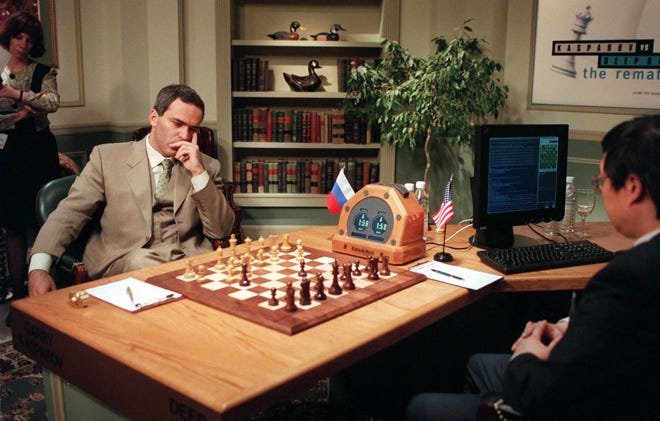
\includegraphics[width=\linewidth]{figure/GKDB.jpg}
            \caption{La celebre partita tra Kasparov e Deep Blue.}
            \label{fig:kasparovAndDeepBlue}
        \end{subfigure}
        \hspace{1cm}
        \begin{subfigure}[b]{0.45\textwidth}
            \centering
            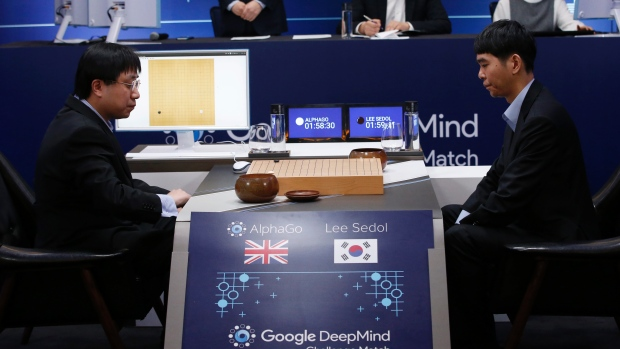
\includegraphics[width=\linewidth]{figure/AGLS.jpg}
            \caption{La storica sfida tra Lee Sedol e AlphaGo.}
            \label{fig:leeSedolAndAlphaGo}
        \end{subfigure}
    \end{tcolorbox}
    \caption{Sfide emblematiche tra esseri umani e intelligenze artificiali.}
    \label{fig:kasparovAndLeeSedol}
\end{figure}

\subsubsection{2017 - AlphaZero}

Nel 2017, DeepMind sviluppa \textbf{AlphaZero}, un sistema generalista capace di imparare a giocare a Go, scacchi e Shogi esclusivamente tramite autoapprendimento, senza l’ausilio di partite umane pregresse. Questo rappresenta un punto di svolta nell’addestramento tramite self-play.

\subsubsection{2017 - Agenti per StarCraft}

Blizzard, in collaborazione con DeepMind, inizia a sviluppare agenti intelligenti capaci di giocare a \emph{StarCraft II}, un gioco particolarmente complesso per via dell’alto numero di azioni e della parziale informazione, segnando questo agente come uno dei primi in assoluto a essere in grado di interagire con un videogioco.

\subsubsection{2016–2019 - OpenAI Five}

Tra il 2016 e il 2019, OpenAI sviluppa \textbf{OpenAI Five}, un agente capace di giocare a \emph{Dota 2}, vincendo contro team professionisti in una modalità 5 contro 5. Si tratta di una delle dimostrazioni più sofisticate di intelligenza artificiale collaborativa.

\subsubsection{2019 - AlphaStar}

Nel 2019, DeepMind introduce \textbf{AlphaStar}, che raggiunge prestazioni da livello campione mondiale in \emph{StarCraft II}, grazie a una combinazione di reinforcement learning, imitazione e tecniche avanzate di training multi-agente.

\subsubsection{2018–2020 - AlphaFold 2}

Tra il 2018 e il 2020, DeepMind sviluppa \textbf{AlphaFold 2}, un sistema rivoluzionario in grado di prevedere la struttura tridimensionale delle proteine con un'accuratezza senza precedenti, partendo dalla sola sequenza amminoacidica.

\subsubsection{2018–2020 - BERT}

Google introduce \textbf{BERT} (Bidirectional Encoder Representations from Transformers), un modello per la comprensione contestuale del linguaggio, che consente una rappresentazione semantica più profonda rispetto ai modelli precedenti.

\subsubsection{2021 - DALL·E}

Nel 2021, OpenAI presenta \textbf{DALL·E}, un modello generativo capace di produrre immagini realistiche a partire da descrizioni testuali.

\subsubsection{2022 - ChatGPT}

Nel 2022, OpenAI introduce \textbf{ChatGPT}, un \textbf{LLM} (Large Language Model) capace di generare risposte coerenti e plausibili, con un’interfaccia conversazionale estremamente naturale, pur con limiti di accuratezza.

\subsubsection{2023 - Bard}

Nel 2023, Google rilascia \textbf{Bard}, un LLM concorrente di ChatGPT. Tuttavia, a causa di alcune imprecisioni e problemi di affidabilità nelle risposte, viene rapidamente ritirato.

\subsubsection{2023 - Gemini}

Sempre nel 2023, Google lancia \textbf{Gemini}, un modello multimodale progettato per gestire contemporaneamente testo, immagini e audio, aprendo la strada a interazioni AI più complesse e versatili.

\begin{center}
    \begin{tikzpicture}[scale=0.75, every node/.style={transform shape, draw, rounded corners, align=center, font=\small, text width=2.5cm}, node distance=0.8cm]
        \node (1997) [fill=red!30] {1997\\Deep Blue};
        \node (2011) [fill=blue!30, below=of 1997] {2011\\Watson};
        \node (2016) [fill=green!30, right=of 2011] {2016\\AlphaGo};
        \node (2017) [fill=yellow!30, below=of 2016] {2017\\AlphaZero};
        \node (2019) [fill=purple!30, right=of 2017] {2019\\AlphaStar};
        \node (2020) [fill=orange!30, below=of 2019] {2020\\AlphaFold 2};
        \node (2021) [fill=cyan!30, right=of 2020] {2021\\DALL·E};
        \node (2022) [fill=pink!30, below=of 2021] {2022\\ChatGPT};
        \node (2023) [fill=gray!30, right=of 2022] {2023\\Bard/Gemini};
        
        \draw[->, thick] (1997) -- (2011);
        \draw[->, thick] (2011) -- (2016);
        \draw[->, thick] (2016) -- (2017);
        \draw[->, thick] (2017) -- (2019);
        \draw[->, thick] (2019) -- (2020);
        \draw[->, thick] (2020) -- (2021);
        \draw[->, thick] (2021) -- (2022);
        \draw[->, thick] (2022) -- (2023);
    \end{tikzpicture}
    
    \vspace{0.5em}
    \textbf{Figura 1:} Evoluzione cronologica dei principali modelli di Deep Learning dal 1997 al 2023.
\end{center}

\subsubsection{Conclusione}

Quelli analizzati finora rappresentano solo una minima parte dell'enorme ecosistema di modelli di Deep Learning sviluppati negli ultimi decenni. Sono stati scelti solo alcuni di essi legati, alla loro rilevanza nel corso del Prof. Anelli. L'esplosione e la diffusione di questi modelli sono dovute a ingenti investimenti specialmente da parte di aziende private ma anche da parte di enti governativi, rendendo l'Intelligenza Artificiale un settore strategico globale. Tutto ciò ci permette di comprendere a grandi linee qual è stata la progressione naturale e i maggiori focus su degli specifici task su cui ci si è soffermati negli ultimi anni da parte dell'AI, in modo da permetterci di capire soprattutto come siamo giunti agli attuali sviluppi.

\section{Aspetti Etici e Sicurezza}

L'espansione dell'intelligenza artificiale ha sollevato specialmente degli interrogativi etici, sociali e legali. Tra le principali preoccupazioni troviamo la sostituzione dell’essere umano in diversi settori lavorativi, la perdita di privacy, i rischi legati alla sicurezza e l’insufficiente trasparenza di molti sistemi. Il ruolo delle istituzioni pertanto, diventa centrale nell'effettuare una giusta regolamentazione, ma anche i ricercatori hanno la responsabilità di considerare le implicazioni etiche delle tecnologie che sviluppano, ovviamente è risaputo come effettuare dei controlli sulla sicurezza porta un dispendio di costi ulteriore e dei rallentamenti dal punto di vista commerciale, e proprio per questo molte aziende che si occupano di ciò sottovalutano questi aspetti concentrandosi principalmente su un fine commerciale.

\subsection{Banche dati esposte}

In diversi casi, database contenenti dei dati biometrici, come il riconoscimento facciale o tattile, sono stati archiviati senza aver adottato in precedenza delle adeguate misure di sicurezza, esponendo i dati sensibili degli utenti a rischi di uso improprio, questa cosa si è venuta a verificare molto spesso in dei contesti autoritari o militari, dunque dei contesti nei quali la perdita di informazioni di una tale sensibilità è notevolmente pericolosa.

\subsection{Bias}

L’intelligenza artificiale può riflettere e amplificare i bias presenti nei dati di addestramento. Un bias è un preconcetto, che una determinata persona può avere, a causa del contesto in cui si è cresicuti e alle cose a cui si è stati esposti, portandola a pensare in una determinata maniera, al di fuori dall'astrazione di una qualsivolgia forma di oggettività, infatti possono esistere delle persone le quali hanno delle ideologie politiche, idee religiose, sociali, culturali diverse, portando a un Bias rilevante nel momento in cui si cerca di giudicare un argomento in maniera quanto più oggettiva possibile. L'inteliggenza artificiale è fortemente condizionata dai Bias, presenti nei dataset sui quali viene allenata, alcuni esempi includono discriminazioni razziali nei modelli di giustizia predittiva o disparità di genere in modelli di selezione automatica del personale.

\subsection{Filter Bubble}
La \textit{filter bubble} (in italiano: bolla di filtraggio) è un concetto sviluppato da Eli Pariser nel suo libro \textit{The Filter Bubble: What the Internet Is Hiding from You (2011)}. Indica un ambiente informativo personalizzato in cui un individuo è esposto principalmente a contenuti che confermano le sue convinzioni preesistenti, mentre informazioni opposte o divergenti vengono filtrate o nascoste da algoritmi online. Una filter bubble si crea quando algoritmi (di Google, Facebook, YouTube, TikTok, ecc\dots) selezionano e mostrano contenuti in base ai tuoi interessi, click, like, cronologia di navigazione, e comportamenti passati, limitando così l’esposizione a idee differenti o contrastanti.

\subsection{Polarization Effect}

Una conseguenza della filter bubble, è sicuramente la polarizzazione, la quale scatena il polarization effect: gruppi omogenei finiscono per rafforzare le proprie opinioni in modo estremo, con conseguente aumento della divisione sociale, come visibile nei dibattiti online su temi sensibili. Questa cosa sicuramente non restituisce un'immagine reale della realtà poiché si vede tutto in maniera polarizzata, per l'appunto, dando pieno valore ai pareri estremi e non valutando tutte le possibili sfumature di grigio le quali possono essere presenti all'interno di un discorso.

\subsection{Adversarial Attacks}

Un \textit{adversarial attack} (in italiano: attacco avversario) è una tecnica utilizzata per ingannare un modello di machine learning, in particolare i modelli di deep learning, introducendo piccole perturbazioni appositamente progettate nei dati di input, tali da causare errori di classificazione o comportamenti indesiderati, senza che l’errore sia evidente a un osservatore umano. Un classico esempio è quello di immaginarsi un modello che classifica correttamente un’immagine come "papera". Se aggiungiamo una perturbazione invisibile all’occhio umano, il modello potrebbe classificare questa papera come "cavallo" con altissima confidenza e sicurezza, pur sembrando a noi ancora un papera (Figura~\ref{fig:adattack}).

\begin{figure}
    \centering
    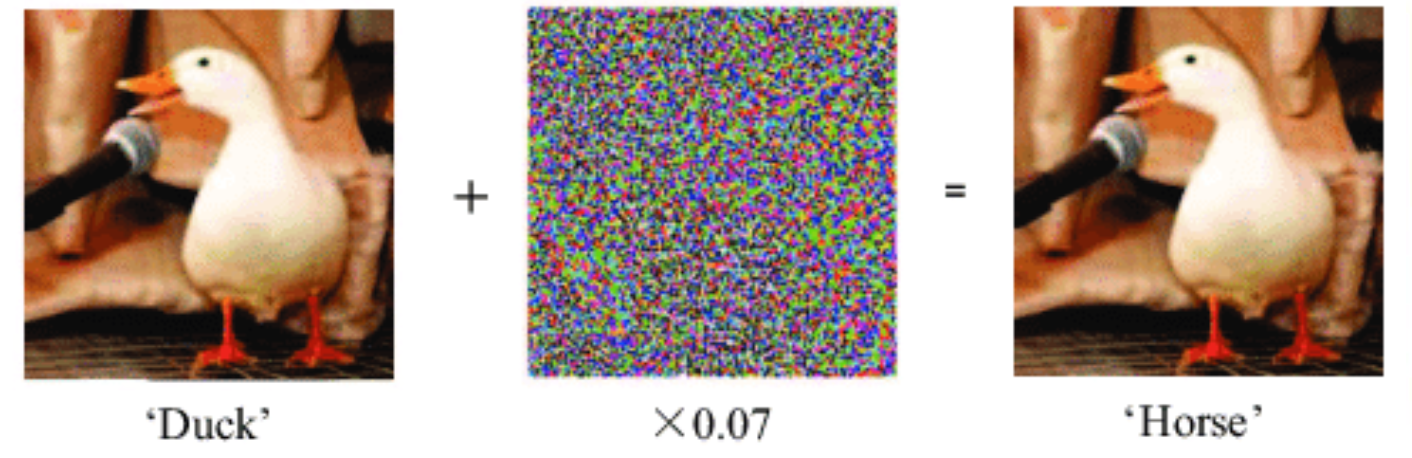
\includegraphics[width=0.75\textwidth]{figure/AdversarialAttack.png}
    \caption{Esempio di Adversarial Attack, in cui una papera viene classificata come cavallo a seguito dell'aggiunta di un rumore esterno.}
    \label{fig:adattack}
\end{figure}

\subsection{Data Poisoning}
Il \textit{data poisoning} è una forma di attacco contro i sistemi di machine learning in cui un attaccante manipola i dati di addestramento allo scopo di compromettere il comportamento del modello durante l’inferenza. Il data poisoning è come "avvelenare il cibo del cervello dell’IA": se il modello impara da dati falsificati o manipolati, finirà per imparare cose sbagliate. Questa tipologia di attacco risulta essere una vera e propria minaccia per la sicurezza e affidabilità dei modelli, soprattutto in contesti critici (sanità, difesa, veicoli autonomi). Questo è anche un ruolo molto critico, difficile da rilevare, specialmente nei modelli addestrati su dati pubblici o crowdsourced (es. GitHub, Kaggle, internet).


\subsection{Federated Learning}

Il \emph{federated learning} è un paradigma che consente l’addestramento distribuito del modello direttamente sui dispositivi degli utenti, migliorando la privacy e riducendo la necessità di centralizzare dati sensibili (Figura~\ref{fig:FedLearning}).

\begin{figure}
    \centering
    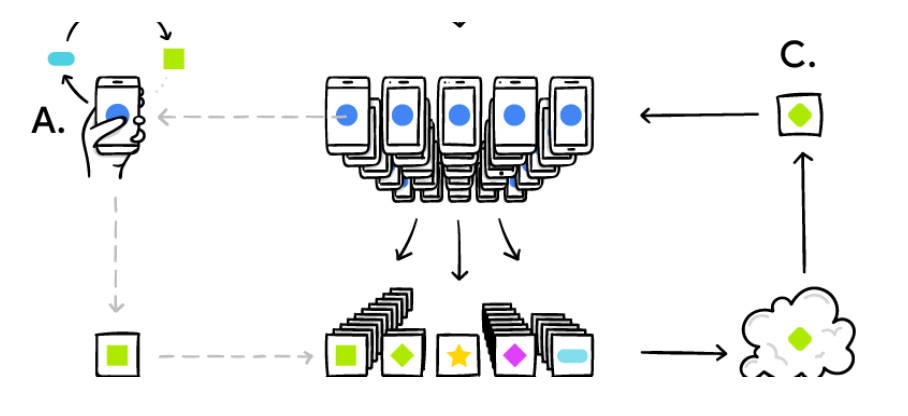
\includegraphics[width=0.85\textwidth]{figure/FederatedLearning.png}
    \caption{Architettura rappresentativa del Federated Learning.}
    \label{fig:FedLearning}
\end{figure}

\subsection{Sostenibilità e AI}

L’addestramento dei modelli di AI comporta un notevole consumo energetico. Ad esempio, GPT-3 ha richiesto risorse ingenti, contribuendo significativamente all’impatto ambientale. È quindi fondamentale sviluppare tecnologie più sostenibili, attraverso hardware efficiente e tecniche di training più leggere.

\subsection{AI Act}

L’\textbf{AI Act} dell’Unione Europea è una proposta legislativa che mira a classificare i sistemi di intelligenza artificiale secondo il livello di rischio. I sistemi ad alto rischio saranno soggetti a requisiti più stringenti, mentre quelli a basso rischio avranno meno restrizioni, promuovendo al contempo trasparenza e responsabilità.
